\documentclass[12pt,oneside,a4paper]{report} 
\usepackage[utf8]{inputenc}
\usepackage[czech]{babel}
\usepackage{graphicx}
\usepackage{fancyhdr}
\usepackage{tabularx}
\usepackage{supertabular}
\usepackage{comment}
% right header      
\rhead{Moon Games}
% left header
\lhead{Collab network protocol}
% centered footer
\cfoot{\thepage}
% use this style
\pagestyle{fancy}

% capter style
\makeatletter
\def\@makechapterhead#1{
{\parindent \z@ \raggedright \normalfont
\interlinepenalty\@M
\LARGE \bfseries \thechapter\ #1\par\nobreak
\vskip 30\p@
}}
\makeatother


\begin{document}

\tableofcontents
\newpage


\part{Úvod}

\section{Licence}

All text of this document is licenced by GNU FDL version 1.3 or greater. Current version text of licence you can find on web address http://www.gnu.org/copyleft/fdl.html.

\section{Tento dokument}

Tento dokument se nachází ve stavu přípravy. Může obsahovat chyby, rozpory nebo neúplné informace. Berte prosím v potaz jeho vývoj a na případné chyby upozorněte autory.

Text of his parts is now in czech language. Please be patient and wait to translation. We are sorry. If you can help us with translation we will be pleasure with us cooperation.

\section{Úvod}

Dokument popisuje síťový protokol ke kolaborativnímu (síťovému) kreslení. V první části popisujeme co za kolaborativní kreslení považujeme, co by mělo a co naopek němelo obsahovat (viz str. \ref{part.colaborative-painting}). Další část se stahuje k vlastnímu protokolu (viz str. \ref{part.protocol}).

\part{Kolaborativní kreslení}
\label{part.colaborative-painting}


\part{Protokol}
\label{part.protocol}


\chapter{Obecný popis}

Collab může komunikovat různými síťovými protokoly, důležite je, aby bylo možné skrze ně v reálném čase posílat tzv. collab message (viz strana \ref{text.collab_message}).

\chapter{Collab message}
\label{text.collab_message}

Collab message je posloupnost bytů, která nese informaci o své délce, příkazu a přídavná data (bloky).

\section{Values}

Pokud není uvedeno jinak, všechny celočíselné hodnoty jsou bezeznaménkové a každý bit má hodnotu $2^{p}$. Kde $p$ je pozice bitu a poslední bit posloupnosti má pozici $0$. Například posloupnost $00001010$ má hodnotu $10$ ($2^1 + 2^3$).

Celočíselné znaménkové a reálné číselné hodnoty dodržují binární ukládání číselných hodnot v Javě (byte, short, int, long, float, double).

Logické hodnoty (boolean) jsou reprezentovány jedním bytem, kde samé nuly ($00000000$) reprezentují hodnotu \emph{false} a hodnota jedna ($00000001$) reprezentuje hodnotu \emph{true}. Ostatní hodnoty jsou považovány za nevalidní.

Veškerý text je kódován jako UTF-8.

\section{Message}

Zpráva začíná čtyřmi byty udávající délku celé zprávy (neznaménkové číslo) bez těchto prních čtyř.

Po načtení délky zprávy se načté právě tolik dalších bytů, které se následně zpracovávají.

Další dva byty (pátý a šestý) jako neznaménkové číslo udávají příkaz (typ) zprávy.

Po typu příkazu následuje seznam bloků (viz strana \ref{text.collab_message.block}), které mohou být v posloupnosti bytů zprávy umístné v libovolném pořadí. Není možné bloky dělit na jednotlivé části (podposloupnosti) a ty jakýmkoli způsobem ve zprávě permutovat!

Obsah message je tedy následující:

\begin{enumerate}
	\item message length (4\,{}B)
	\item command (2\,{}B)
	\item blocks (message length - 2 B)
\end{enumerate}

Obsah zprávy je také ilustrován diagramem \ref{picture.message_structure}.

\begin{figure}[h]
  \centering
  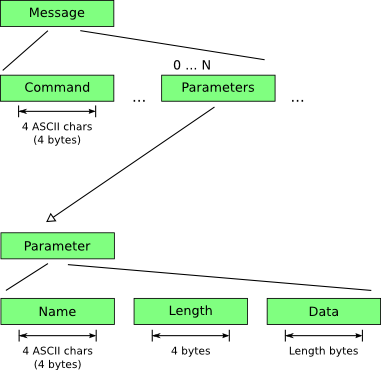
\includegraphics[width=0.80\textwidth]{diagrams/message_structure_diagram.png}
  \caption{Message structure diagram}
  \label{picture.message_structure}
\end{figure}

\section{Block}
\label{text.collab_message.block}

Blok se dělí na tři části v následujícím pořadí.

\begin{enumerate}
	\item block type (1\,{}B)
	\item block length (2\,{}B)
	\item block data (block length\,{}B)
\end{enumerate}

Block type identifikuje blok, je to jednobytové neznaménkové číslo.

Block length udává délku dat bloku (nezahrnuje první dvě části bloku). Je to dvoubajtové neznaménkové číslo.

Block data obsahuje data bloku.

\chapter{Commands}

Příkazy se dělí na příchozí (posílá je server na klienty), odchozí (klienti je posílají na server) a obousměrné.

Seznam příkazů a jejich číselných hodnot:

\begin{itemize}
	\item Paint: 1
	\item Layers order: 12
	\item Add layer: 11
\end{itemize}

\section{Příchozí}

\section{Odchozí}

\subsection{Add layer}

Přidá vrstvu do plátna. Obsahuje tyto bloky:

\begin{itemize}
	\item Layer position: 1
	\item Layer name: 2
	\item Canvas ID: 3
\end{itemize}

\paragraph{Layer position}
Obsahuje celočíselné čtyřbytové bezznaménkové číslo, které udává kolikátá v pořadí bude vrstva od spoda po přidání. Vrstva na pozici $0$ bude pod všemi ostatními.

\paragraph{Layer name}
Obsahuje text s názvem vrstvy.

\paragraph{Canvas ID}
Obsahuje celočíslené bezznaménkové čtyřbytové číslo s ID plátna, do kterého má být vrstva přidána.

\section{Obousměrné}

\subsection{Paint}

Tento příkaz informuje o aktualizaci kreslícího plátna. Obsahuje tyto bloky:

\begin{itemize}
	\item Update type: 1
	\item Update ID: 2
	\item Layer ID: 3
	\item Canvas ID: 4
	\item X coordinate: 5
	\item Y coordinate: 6
	\item Update image data: 7						
\end{itemize}

\paragraph{Update type}
Update type je typ updatu a obsahuje čtyřbytové neznaménkové celočíselné číslo udávající typ updatu. Může nabívat hodnot $0$ a $1$, kde $0$ reprezentuje přidávácí update a $1$ mazací.

V případě přidávacího updatu se standartním (source over) algoritmem update nakreslí přes obrázek vrstvy. 

V případě odebíracího updatu se jen mění velikost alpha kanálu jednotlivých pixelů updatované vrstvy. Výsledná alpha každého pixelu $D_{a}$ se spočítá jako $D_{a} = S_{a} \cdot P_{a}$ kde $S_{a}$ značí alphu pixelu v updatovacím obrázku a $P_{a}$ značí alphu v v obrázku vrstvy před updatem. Všechny alphy ve výpočtu nabívají hodnot $0$ až $1$, takže je před výpočtem potřeba je převést ze standartní podoby $0$ až $255$ na tyto dělením číslem $255$ a po výpočtu převést zpátky násobením.

\paragraph{Update ID}
Obsahuje čtyřbytové neznaménkové celé číslo, které identifikuje tento update.

\paragraph{Layer ID}
Obsahuje čtyřbytové neznaménkové celé číslo, které identifikuje updatovanou vrstvu.

\paragraph{Canvas ID}
Obsahuje čtyřbytové neznaménkové celé číslo, které identifikuje updatované kreslící plátno (je tak možné kreslit na několik pláten).

\paragraph{X coordinate}
Obsahuje čtyřbytové neznaménkové celé číslo, které udává X souřadnici levého horního rohu updatu (kam se aplikuje updatovací obrázek).

\paragraph{Y coordinate}
Obsahuje čtyřbytové neznaménkové celé číslo, které udává Y souřadnici levého horního rohu updatu (kam se aplikuje updatovací obrázek).

\paragraph{Update image data}
Obsahuje binární data PNG obrázku typu ABGR. Viz http://www.w3.org/Graphics/PNG/. 

\end{document}